\newpage
%**************************************************************
\chapter{Analisi dei requisiti}
\label{cap:analisi-requisiti}
La prima attività per la definizione del prodotto da sviluppare è l'analisi dei requisiti.
\\
Dopo aver preso confidenza con gli strumenti base da utilizzare e le norme aziendali da applicare, ho partecipato ad un incontro con il tutor aziendale ed il committente del progetto, durante il quale è stata discussa una presentazione predisposta dal committente, che enunciava lo scopo e le funzionalità considerate inizialmente per il prodotto.
\\
Tale presentazione ha segnato l'avvio dell'attività di analisi dedicata al progetto dello stage e ha descritto una prima serie di specifiche.
\\
L'analisi dei requisiti è stata quindi dettagliatamente illustrata in un format appositamente predisposto dall'azienda, nel quale era richiesto di specificare lo scopo del prodotto, il contesto in cui potesse essere inserito, i vantaggi attesi, i requisiti relativi, i casi d'uso ed eventuali diagrammi aggiuntivi.
\section{Requisiti}
\subsection{Struttura}
Ho inizialmente suddiviso in due liste: \textbf{funzionali} e \textbf{non funzionali}, per limitarne la complessità, in quanto l'applicativo oltre a offrire delle funzionalità all'utente. deve anche rispettare le caratteristiche delle applicazioni mobile imposte dall'azienda.
\\
Ho descritto i requisiti con frasi brevi e concise, per rendere più evidenti le funzionalità di cui deve disporre il prodotto.
\\

\subsection{Acquisizione}
Ho potuto definire progressivamente i requisiti del prodotto richiesti dall'Azienda nel corso delle riunioni con il tutor aziendale ed il committente. \\
Durante la prima riunione abbiamo discusso le funzionalità dell'applicativo mobile, le specifiche richieste dal committente e lo stile grafico che l'applicativo dovrà mantenere, consentendomi di approntare una prima lista di requisiti per il nuovo prodotto. \\
In riunioni successive, abbiamo discusso i requisiti ottenuti e le funzionalità prese in considerazione. Mi sono stati segnalati eventuali requisiti spiegati in modo superficiale o poco comprensibili, in modo da correggere il contenuto per ittenere un'analisi di buona qualità.
\subsection{Risultati}
Nella redazione conclusiva sull'individuazione dei requisiti ho quindi definito quali erano le funzionalità dell'applicativo, creando dei mockup per stabilire le impostazioni grafiche e definendo i casi d'uso principali.
\section{Casi d'uso}
Per rendere più evidenti le funzionalità proposte dall'applicativo e per meglio definire quali fossero le azioni consentite dagli utenti ad ogni utilizzo, ho preparato una serie di casi d'uso, la cui definizione deriva dai requisiti ottenuti e dalle discussioni sulle caratteristiche del prodotto con il tutor aziendale ed il committente. \\
Per i casi d'uso creati ho previsto soltanto due \textit{attori\ped{G}}. Utente e Utente identificato; questa divisione è risultata necessaria per lo scopo dell'applicativo, perché prevede sia l'utilizzo di un utente con un account aziendale, sia l'utilizzo di un utente senza account, dunque con funzionalità solo \textit{offline}. \\
Ogni caso d'uso rappresenta la schermata dell'applicativo in cui un utente si può trovare e le azioni consentite in quella schermata, correlando ogni schema con una descrizione di quello che compare sul display ed una definizione dettagliata delle opzioni disponibili.
\begin{figure}[ht]
	\centering
	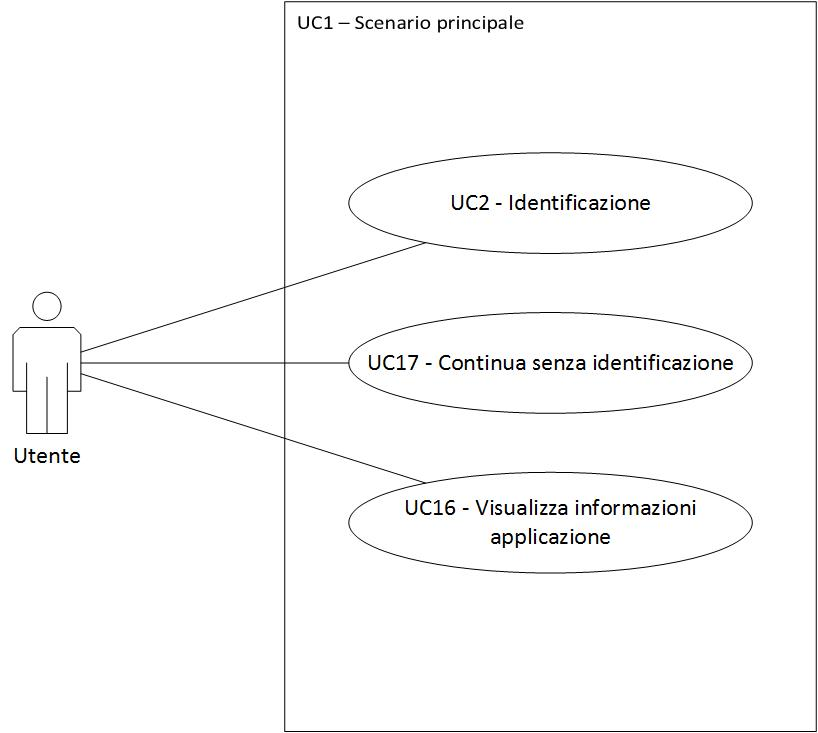
\includegraphics[scale=0.35]{immagini/analisi/UC01_scenario_principale.jpg}
	\caption{\textit{Schema UML Pagina di identificazione}}
\end{figure}\FloatBarrier

\begin{figure}[ht]
	\centering
	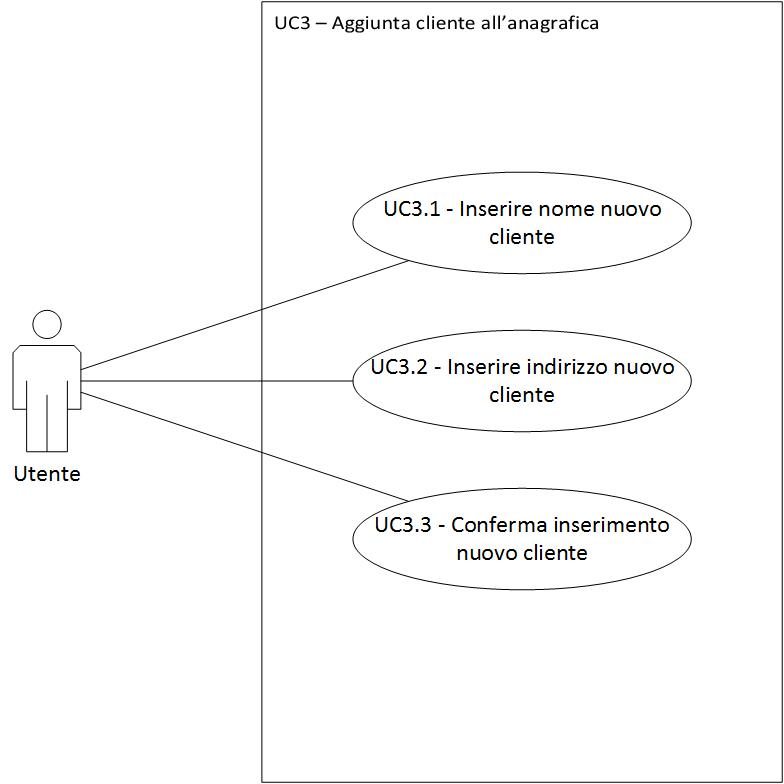
\includegraphics[scale=0.35]{immagini/analisi/UC03_aggiunta_cliente_anagrafica.jpg}
	\caption{\textit{Schema UML Pagina di aggiunta anagrafica cliente}}
\end{figure}\FloatBarrier


\section{Diagrammi di Attività}
Come parte finale dell'analisi dei requisiti ho presentato dei diagrammi di attività per chiarire il flusso di attività intrapreso dall'applicativo in varie schermate: di seguito un esempio di diagramma creato durante l'attività di analisi:

\begin{figure}[ht]
	\centering
	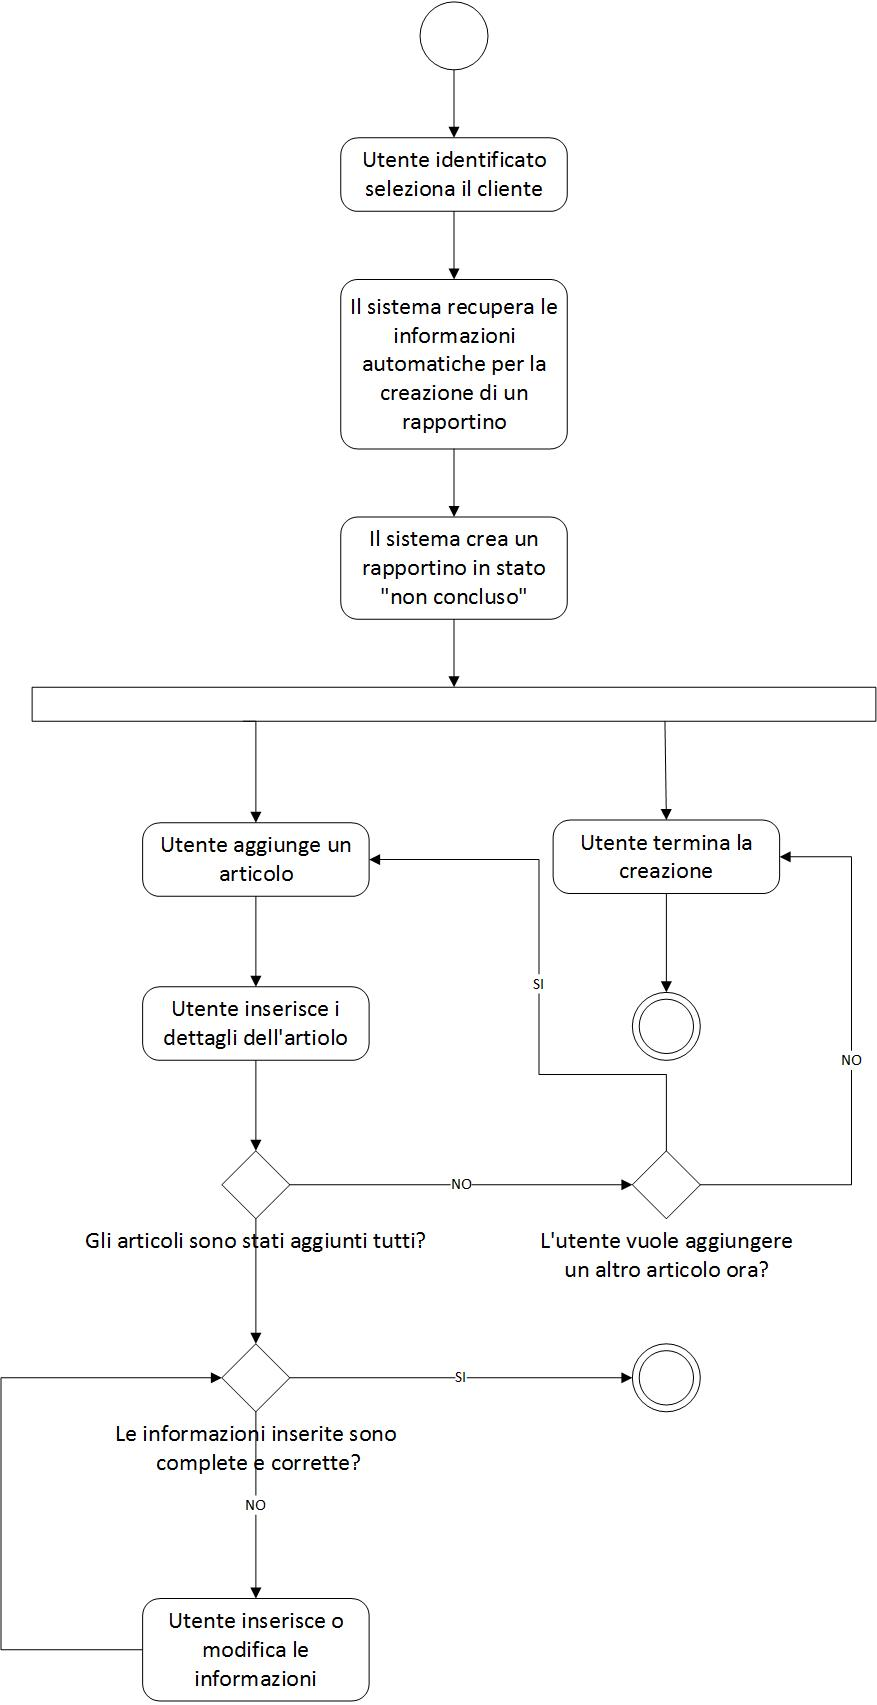
\includegraphics[scale=0.52]{immagini/analisi/003_creazione_rapportino.jpg}
	\caption{\textit{Diagramma Attività di creazione del rapportino}}
\end{figure}\FloatBarrier



